\section{Zielsetzung}
Durch das Verfahren des optischen Pumpens ist es möglich, eine Umkehr in den Besetzungszahlen
zu erzeugen. Damit können mit hoher Präzision die Energeiaufspaltungen der Hyperfeinstruktur oder
der Zeemanaufspaltung, die durch die Anlage eines äußeren Magnetfeldes hervorgerufen werden,
gemessen werden. Hieraus lassen sich die Landéschen g-Faktoren und der
Spin der Elektronenhülle und des Kerns bestimmen.
Konkret werden im Versuch die beiden Rubidiumisotope $^{85}$Rb und $^{87}$Rb untersucht.

\section{Theorie}
\label{Theorie}
Während die innersten Elektronenschalen nach dem Pauliprinzip vollständig besetzt
werden, so erfolgt die Besetzung der äußeren Schalen temperaturabhängig.
Für die zwei Zustände mit den Energien $W_1$ und $W_2$ und den Besetzungszahlen $N_1$ und
$N_2$ gilt für das Verhältnis zwischen den Besetzungszahlen die Boltzmann'sche Gleichung:
\begin{align*}
    \frac{N_{2}}{N_{1}} = \frac{g_{2}}{g_{1}}\frac{\exp(-W_{2}/\text{kT})}{\exp(-W_{1}/\text{kT})} \; .
\end{align*}
Die Größen $g_{\text{i}}$ geben hierbei die Anzahl der zu den Energien $W_1$ und $W_2$ gehörenden
Zustände an.
Mittels des Verfahrens des optischen Pumpens ist es möglich, dieses Verhältnis zu verändern
oder gar zu invertieren ($N_{2} > N_{1}$).


\subsection{Energieaufspaltung}
In einem Atom können sich dessen Energieniveaus auf unterschiedliche Weise aufteilen.
In einer ersten Näherung soll zunächst der Fall betrachtet werden, in dem davon ausgegangen wird, der
Kernspin sei Null.
Der Gesamtdrehimpuls der Valenzelektronen des Atoms $\vec{\text{J}}$ erzeugt hierbei
ein magnetisches Moment $\vec{\mu}_{\text{J}}$, welches wie folgt definiert ist:
\begin{align*}
    \vec{\mu}_{\text{J}} &= -\text{g}_{\text{J}} \cdot \mu_{\text{B}} \cdot \vec{\text{J}} \\
    |\vec{\mu}_{\text{J}}| &= \hspace{1em} \text{g}_{\text{J}} \cdot \mu_{\text{B}} \cdot \sqrt{ \text{J} (\text{J}+1) }
\end{align*}
Hier beschreibt $\mu_{\text{B}}$ das Bohr'sche Magneton.
Der Landé-Faktor $\text{g}_{\text{J}}$ dient zur Berücksichtigung des Umstandes, dass sich der Gesamtdrehimpuls aus dem Bahndrehimpuls $\vec{\text{L}}$ und dem Spin $\vec{\text{S}}$ desr Valenzelektronen zusammensetzt.
Für die magnetischen Momente, die durch Spin und Bahndrehimpuls hervorgerufen werden $\vec{\mu}_{\text{L,S}}$, gilt:
\begin{align*}
    |\vec{\mu}_{\text{L}}| &= \mu_{\text{B}} \sqrt{\text{L} (\text{L}+1)} \\
    |\vec{\mu}_{\text{S}}| &= \text{g}_{\text{S}} \cdot \mu_{\text{B}} \sqrt{\text{S}(\text{S}+1)} \; .
\end{align*}
Vektoriell beschrieben, sieht die Kopplung der magnetischen Momente, die aus dem Spin und dem Bahndrehimpuls resultieren wie folgt aus:
\begin{align*}
    \vec{\mu}_{\text{J}} &= \vec{\mu}_{\text{L}} + \vec{\mu}_{\text{S}} \\
    |\vec{\mu}_{\text{J}}| &= |\vec{\mu}_{\text{L}}| \cos(\beta) + |\vec{\mu}_{\text{S}}| \cos{\alpha} \; .
\end{align*}
Nun lässt sich mit Hilfe des Cosinussatzes, angewendet auf das Dreieck, das von $\vec{\mu}_{\text{L}}, \vec{\mu}_{\text{J}} \text{und} \vec{\mu}_{\text{S}}$ aufgesapnnt wird, eine Formel zur Berechnung des Landé-Faktors herleiten:
\begin{align}
    \text{g}_{\text{J}} = \frac{(\text{g}_{\text{s}} + 1) \cdot \text{J} (\text{J} + 1) + (\text{g}_{\text{s}}-1) \cdot \left[\text{S}
    \cdot (\text{S}+1) - \text{L} (\text{L} + 1) \right]}{2 \cdot \text{J} (\text{J} +1 )}
    \label{eq:La-Fa.gj}
\end{align}
Beim Anlegen eines äußeren Magnetfeldes B, kommt es zur Aufspaltung der Energieniveaus, was als Zeeman-Effekt bekannt ist. Die Energie der magnetischen Wechselwirkung wird wie folgt beschrieben:
\begin{align}
    E_{\text{mag}} &= \vec{\mu}_{\text{J}} \cdot \vec{\text{B}} \\
    &= \text{M}_\text{J} \cdot \text{g}_\text{J} \cdot \mu_{\text{B}} \cdot \text{B} \; .
    \label{eq:E_mag}
\end{align}
Hierbei gilt für die Orientierungsquantenzahl $\text{M}_\text{J}$ auf Grund der Richtungsquantelung: $\text{M}_{\text{J}} \in [-\text{J}, -\text{J}+1,\hdots,\text{J}-1,\text{J}]$ .

\noindent Folgend wird der Fall betrachtet, in denen der Kernspin nicht verschwindet.
Bei hinreichend schwachem Magnetfeld, wovon im Falle des Versuches ausgegangen werden kann, koppeln der Gesamtdrehimpuls der Elektronenhülle $\vec{\text{J}}$ und der Kernspin $\vec{\text{I}}$ vektoriell aneinander zu einem Gesamtdrehimpuls $\vec{\text{F}}$ des Atoms:
\begin{align*}
    \vec{\text{F}} = \vec{\text{I}} + \vec{\text{J}} \; .
\end{align*}
Durch den Kernspin, spalten sich die Energieniveaus in die Hyperfeinstruktur auf.
Die Anzahl der Niveaus wird durch $2\text{J}+1$ oder $2\text{I}+1$ ermittelt, je nachdem, ob J größer als I ist oder anders herum.
Die Aufspaltung eines Niveaus kann mit Hilfe der Quantenzahl F bestimmt werden, die von I+J bis $|\text{I}-\text{J}|$ läuft. Sie ist als Index für die Niveaus der Hyperfeinstruktur zu betrachten.
Die Hyperfeinstruktur kann wiederum in $2\text{F}+1$ Zeeman-Niveaus aufgespalten werden, indem ein äußeres Magnetfeld angelegt wird.
Eine Beispielhafte Aufspaltung ist in Abbildung \ref{abb:Aufspaltung} zu sehen.
\FloatBarrier
\begin{figure}
    \centering
    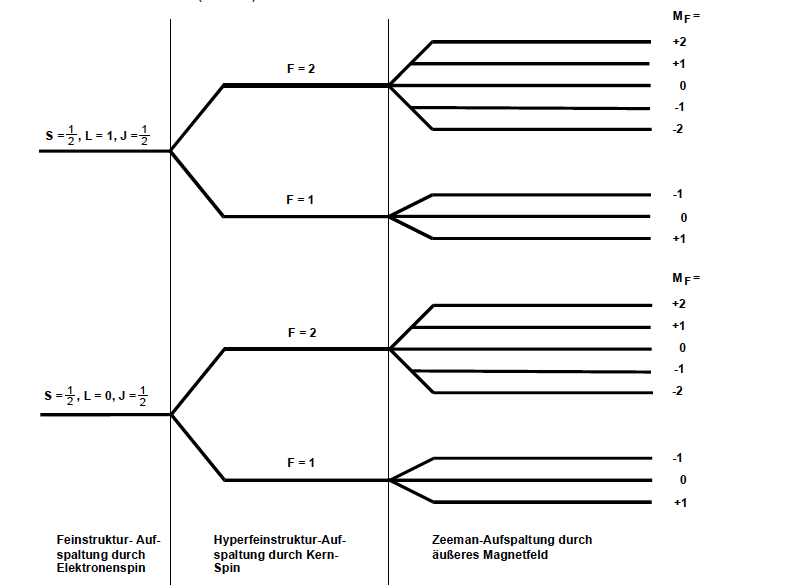
\includegraphics[width=0.7\textwidth]{Aufspaltung.PNG}
    \caption{Aufspaltung der Energieniveaus eines Alkaliatoms mit I = $\frac{3}{2}$ und J = $\frac{1}{2}$ auf Grund von Elektronenspin, Kernspin und externem Magnetfeld. \cite{Q1}}
    \label{abb:Aufspaltung}
\end{figure}
\FloatBarrier
Zwischen zwei benachbarten Energieniveaus herrscht eine Energiedifferenz, die wie folgt berechnet werden kann:
\begin{align*}
    E_{\text{HF}} = \text{g}_{\text{F}} \mu_{\text{B}} \text{B} \; .
\end{align*}
Mittels vektorieller Betrachtung lässt sich der Landé-Faktor $\text{g}_{\text{F}}$ für das Atom bestimmen:
\begin{align*}
    |\vec{\mu}_{\text{F}}| &= \text{g}_{\text{F}} \cdot \mu_{\text{B}} \sqrt{\text{F} (\text{F}+1)} \\
    &=\text{g}_{\text{J}} \cdot \mu_{\text{B}} \sqrt{\text{J} (\text{J} + 1)} \cdot \cos\left(\measuredangle(\vec{\text{J}},\vec{\text{F}})\right) +
    \text{g}_{\text{I}} \cdot \mu_{\text{K}} \sqrt{ \text{I}(\text{I}+1) } \cdot \cos\left(\measuredangle(\vec{\text{I}},\vec{\text{F}})\right) \; .
\end{align*}
Hierbei beschreibt $\mu_{\text{K}}$ das magnetische Moment des Kerns und $\text{g}_{\text{I}}$ den zugehörigen Landé-Faktor.
Allerdings ist auf Grund der großen Massendifferenz zwischen Elektron und Nukleon ( $\rightarrow \mu_{\text{K}} \ll \mu_{\text{B}} $ ) zu beachten, dass in obiger Gleichung der zweite Summand zumeist vernachlässigt wird, womit für den Landé-Faktor folgendes gilt:
\begin{align}
    \text{g}_{\text{F}} \approx \text{g}_{\text{J}} \frac{\text{F} (\text{F} + 1)+\text{J} (\text{J} + 1) - \text{I}(\text{I} + 1)}{2\text{F}(\text{F}+1)} \; .
	\label{eq:La-Fa.gf}
\end{align}

\subsection{Optisches Pumpen}
Wie bereits im Kapitel \ref{Theorie} erwähnt, kann die Besetzung höherer Energieniveaus mit Hilfe der Boltzmannstatistik beschrieben werden.
Mit Hilfe des Verfahrens des optischen Pumpens ist es möglich diese Verteilung zu invertieren, also eine größere Bestzung eines höheren Energiezustandes zu erzeugen.
Um von einem Atom absorbiert zu werden, benötigt ein Photon folgende Energie:
\begin{align*}
    hf = W_{2} - W_{1}
\end{align*}
Diese Energie entspricht der Energie des Photons, was bei einem Übergang von $W_{2}$ auf $W_{1}$ frei würde.
Zunächst wird ein hypothetisches Alkaliatom betrachtet, welches ein Valenzelektron und keinen Kernspin besitzt.
Der Grundzustand dieses Atoms ist druch ${}^2S_{{}^1\!/\!_2}$ und die ersten beiden angeregten Zustände sind durch ${}^2P_{{}^1\!/\!_2}$ und ${}^2S_{{}^3\!/\!_2}$ gegeben. Wie in Abbildung \ref{abb:Aufspaltung2} zu sehen, entstehen durch optische Übergänge zwischen diesen Zuständen zwei Linien: $D_{1}$ und $ D_{2} $.
Der Gesamtspin J der Zustände ${}^2S_{{}^1\!/\!_2}$ und ${}^2P_{{}^1\!/\!_2}$ beträgt $\text{J}= {}^1\!/\!_2$. Daraus ergeben sich für die Orientierungsquantenzahl $\text{M}_\text{J}$ folgende mögliche Werte für die Aufspaltung und für die Differenz $\Delta \text{M}_\text{J}$:
\begin{align*}
    \text{M}_\text{J} &= \pm \frac{1}{2} \\
    \Delta \text{M}_\text{J} &= 0, \pm 1 \; .
\end{align*}
\FloatBarrier
\begin{figure}
  \centering
  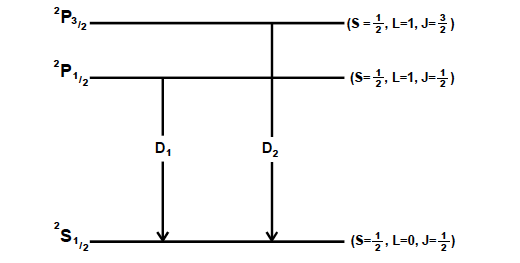
\includegraphics[scale=0.4]{Aufspaltung2.PNG}
  \caption{Dublettstruktur des Alkali-Atoms mit zugehörigen Quantenzahlen. \cite{Q1}}
  \label{abb:D1D2}
\end{figure}
\begin{figure}
  \centering
  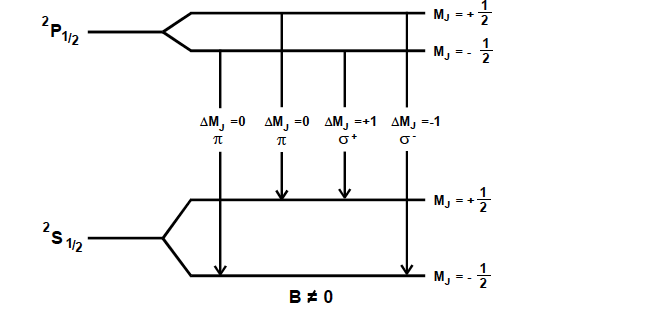
\includegraphics[scale=0.4]{Aufspaltung3.png}
  \caption{Zeeman-Aufspaltung des Grundniveaus und des ersten angeregten Zustands mit möglichen Übergängen des hypothetischen Alkaliatoms\cite{Q1}}
  \label{abb:Aufspaltung2}
\end{figure}
%\begin{figure}
%    \centering
%    \begin{subfigure}{0.8\textwidth}
%        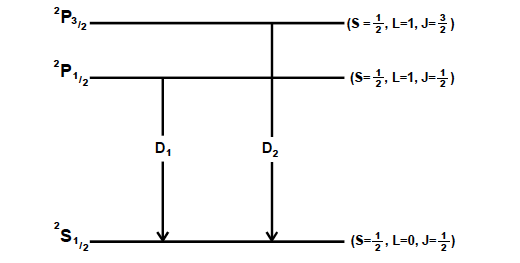
\includegraphics[width=0.49\textwidth, height=0.3\textwidth]{Aufspaltung2.PNG}
%        \subcaption{Dublettstruktur des Alkali-Atoms mit zugehörigen Quantenzahlen. \cite{Q1}}
%        \label{abb:D1D2}
%    \end{subfigure}
%    \begin{subfigure}{0.8\textwidth}
%        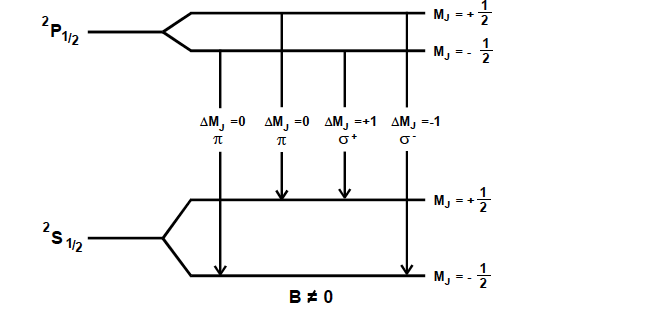
\includegraphics[width=0.40\textwidth, height=0.3\textwidth]{Aufspaltung3.PNG}
%        \caption{Zeeman-Aufspaltung des Grundniveaus und des ersten angeregten Zustands mit möglichen Übergängen des hypothetischen %Alkaliatoms\cite{Q1}}
%        \label{abb:Aufspaltung2}
%    \end{subfigure}
%\end{figure}
\FloatBarrier
Durch Anlage eines externen Magnetfeldes, spalten sich die Grundniveaus und der erste angeregte Zustand auf und es sind gemäß den Auswahlrgelen $\Delta \text{M}_{\text{J}} = 0, \pm1$ Übergänge zwischen den Niveaus möglich, wie in Abbildung \ref{abb:Aufspaltung2} zu sehen ist.
Je nach dem, welcher Übergang stattfindet, ist das dabei emittierte Licht unterschiedlich polarisiert.
Beim $\sigma^+$-Übergang ( $\Delta \text{M} = +1$ ) ist der Spin der emittierten Lichtquanten antiparallel zur Ausbreitungsrichtung und es entsteht rechts zirkular-polarisiertes Licht. Beim $\sigma^-$-Übergang ( $\Delta \text{M} = -1$ ) hingegen sind Spin und Ausbreitungsrichtung parallel. Die beiden $\sigma$-Übergänge werden entlang des Magnetfeldes emittiert, wohingegen der $\pi$-Übergang ( $\Delta \text{M} = +0$ ) senkrecht zum Magnetfeld abgestrahlt wird, wo das Intensitätsmaximum auftreten, und linear polarisiertes Licht emittiert wird.
Nun besteht die Möglichkeit ein Gas aus diesem hypotetischen Alkali-Atom, das sich im thermischen Gleichgewicht befindet,
mit rechts zirkular polarisiertem Licht ($D_1$-Licht) anzuregen und ein äußeres Magnetfeld anzulegen. Da die Orientierungsquantenzahl M hierbei nur +1 oder -1 betragen kann, sind nur Übergänge von ${}^2S_{^1\!/\!_2}$ mit  $M_J=-^1\!/\!_2$ nach ${}^2P_{^1\!/\!_2}$, $M_J=+^1\!/\!_2$ möglich.
Der Übergang vom ersten angeregten Zustand ${}^2P_{^1\!/\!_2}$ mit $M_J=+^1\!/\!_2$ zurück in den Grundzustand findet hierbei durch spontane
Emission statt. Dabei wird sowohl der Grundzustand mit $M_J=-^1\!/\!_2$
als auch der mit $M_J=+^1\!/\!_2$ besetzt. Diese beiden Vorgänge sorgen dafür, dass der energetisch niedrigere Zustand entgegen der thermischen Verteilung, immer weniger besetzt ist und sozusagen "leer" gepumpt wird.
Je weniger der energetisch niedrigere Zustand besetzt ist, umso weniger Lichtquanten werden absorbiert. Mit einem Photodetektor kann ein Maximum des anregenden $D_1$-Lichts gemessen werden. Die gemessene
Transmission nähert sich in der Theorie asymptotisch dem Wert 1, der nur erreicht werden kann, falls es gelingt, den niedrigeren Zustand mit $M_J=-^1\!/\!_2$ völlig leer zu pumpen. Jedoch geht auch durch Streuung Intensität verloren, weshalb es unmöglich sein wird, eine Maximale Intensität von 1 mit dem Photodetektor zu bestimmen.

\subsection{Resonanzstellen}
Durch Anlage eines frequenzvariablen Hochfrequenzfeldes (RF) an die Dampfzelle, wird ein externes Magnetfeld erzeugt. So findet das optische Pumpen statt und es kommt zur oben beschriebenen Besetzungsinversion und in Folge dessen zu einer höheren Transmission des $D_1$- Lichtes.
Im Falle, dass die Energie eines eintreffenden Photons der Energiedifferenz der Zeeman-Aufspaltung entspricht, so kommt es zur induzierten Emission, was wiederum dazu führt, dass das energieärme Besetzungsniveau ${}^2S_{{}^1\!/\!_2}$, $M=-^1\!/\!_2$ wieder aufgefüllt wird, weshalb die Transparenz des Gasgemisches abnimmt und weniger Photonen den Detektor erreichen. Die Theoriekurve in Abbildung \ref{abb:Resonanz} zeigt ein lokales Minimum an der Resonanzstelle $\text{B}_{\text{m}}$.
Die Magnetfeldstärke an der Resonanzstelle berechnet sich wie folgt:
\begin{align}
  \label{eq:2}
    h \nu &= E_{\text{HF}} = \mu_{\text{B}} \text{g}_{\text{J}} \cdot \text{B}_{\text{m}} \\
    \text{B}_{\text{m}} &= \frac{4\pi m_0}{e_0 \text{g}_{\text{J}}}f \; .
\end{align}
\FloatBarrier
\begin{figure}
    \centering
    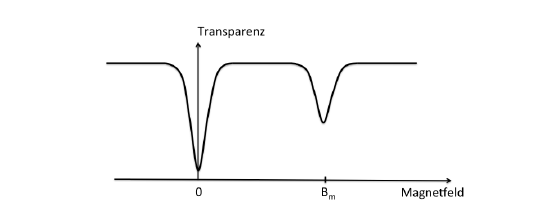
\includegraphics[width=0.8\textwidth]{Resonanz.PNG}
    \caption{Resonanzstellen des Alkali-Atoms in Abhängigkeit vom angelegten Magnetfeld. \cite{Q1}}
    \label{abb:Resonanz}
\end{figure}
\FloatBarrier
Das erste Minimum der Transparenz liegt bei $\text{B}=0$, was daran liegt, dass es durch das Fehlen des Magnetfeldes zu keiner Aufspaltung der Spektrallinien und somit auch zu keinen induzierten Übergängen zwischen den Niveaus kommt und folglich auch das optische Pumpen nicht funktionieren kann.
In diesem Bereich ist der Einfluss des Erdmagnetfeldes zu bestimmen und mit dem angelegten Magnetfeld auszugleichen.

\subsection{Betrachtung für nicht verschwindende Kernspins}
Der Kernspin sorgt für weitere Aufspaltungen der Zeeman-Niveaus.
Wird dieses System mit rechts zirkular polarisiertem Licht bestrahlt, so kommt
es zu Übergängen mit $\Delta \text{M}_{\text{F}} = +1$.
Dies wiederum hat zur Folge, dass nach Beendigung des Pumpvorgangs lediglich der Zustand $\text{F}=2$ mit $M_F=+2$ besetzt sein wird. Von hier aus kann kein Übergang mehr induziert werden, da kein Niveau mit $\text{M}_{\text{F}}=+3$ existiert und dieser Zustand lediglich durch spontane Emission immer weiter besetzt werden kann.
Somit wird auch hier das Grundniveau "leer gepumpt".

\subsection{Quadratischer Zeeman-Effekt}
Bei stärkeren Magnetfeldern, müssen bei der Berechnung von $E_{\text{HF}}$ Terme höherer Ordnung berücksichtigt werden.
Durch das Lösen der Eigenwertgleichung
\begin{align*}
    H \Psi = E \Psi
\end{align*}
unter Berücksichtigung der magnetischen Momente $\vec{\mu}_{\text{J}}$ und $\vec{\mu}_{\text{I}}$, wird die
Energie abhängig von
der  Orientierungsquantenzahl $\text{M}_{\text{F}}$. Die Energie für den Übergang von $\text{M}_{\text{F}}$
nach $\text{M}_{\text{F-
1}}$ lässt sich wie folgt beschreiben:
\begin{align}
  \label{eq_qZeeman}
    E_{\text{HF}} &= \text{g}_{\text{F}} \mu_{\text{B}} B+ \text{g}_{\text{F}}^2 \mu_{\text{B}}^2 B^2
    \frac{1- \text{M}_{\text{F}}}{\Delta E_{\text{Hy}}}- \cdots  \; .
\end{align}
Hierbei ist $E_{\text{Hy}}$ ist die Energiedifferenz der Niveaus F und F$+1$.
\newpage
\section{Durchführung}
\FloatBarrier
\begin{figure}
    \centering
    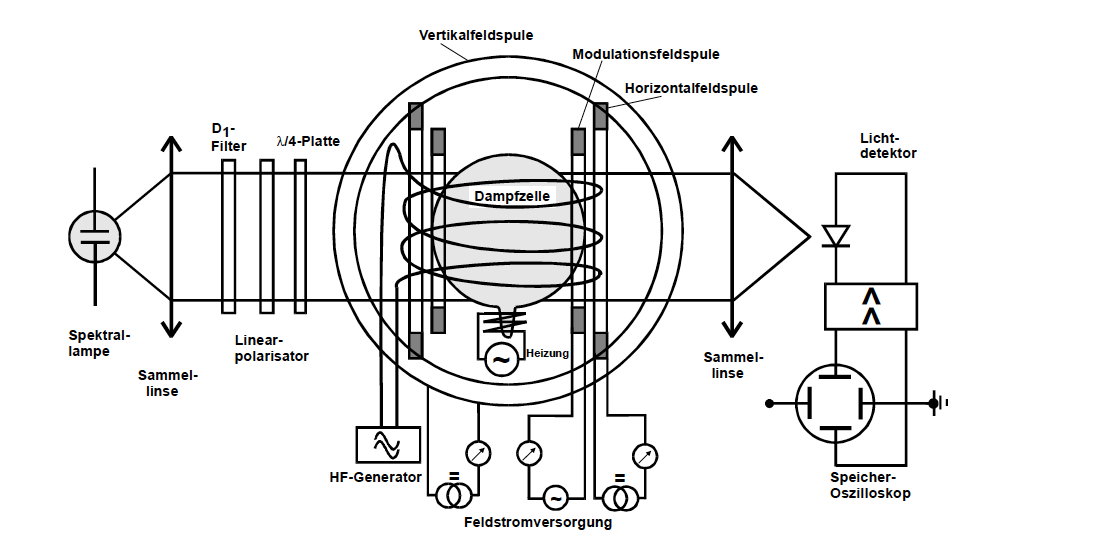
\includegraphics[width=0.9\textwidth]{Aufbau.PNG}
    \caption{Schematischer Versuchsaufbau}
    \label{abb:Aufbau}
\end{figure}
\FloatBarrier
Der schematische Versuchsaufbau ist in Abbildung \ref{abb:Aufbau} zu sehen.
Zunächst durchläuft das Licht der Rubidiumdampflampe eine Kollimationslinse, die das Licht bündelt. Darauf
folgt
ein sogenannter $\text{D}_1$-Filter, der den Lichtstrahl so filtert, dass
lediglich die $\text{D}_1$-Linie aus dem Rubidiumspektrum mit einer Wellenlänge von
$\SI{794,8}{\nano\meter}$ hindurchgelassen wird.
Der Linearpolarisator, der dahinter aufgestellt ist, macht aus dem unpolarisierten
Lichtstrahl zunächst linear polarisiertes Licht, welches durch den $\lambda\:/\:4$-Filter zu rechts polarisiertem Licht
wird.
Der gebündelte Lichtstrahl durchläuft darauf hin eine Dampfzelle, in der sich $^{85}$Rb
und $^{87}$Rb Isotope als Gemisch befinden. Zwischen Dampfzelle und Photodiode befindet
sich abermals eine Sammellinse, um den Lichtstrahl auf den Eingang der Photodiode zu fokussieren. Die Photodiode ist mit
einem Oszillospkop verbunden, welches in
Abhängigkeit von der gemessenen Intesität einen Ausschlag in y-Richtung anzeigen wird.

\noindent Um die Zelle herum befinden sich zwei Helmholtzspulenpaare. Eine, um das vertikale Erdmagnetfeld auszugleichen. Um die
Spule, die ein horizontales Magnetfeld
erzeugt, ist eine weitere Spule, die Sweep-Spule, gewickelt. Diese beiden Spulen werden
benötigt, um die Zeeman-Aufspaltung der Energieniveaus hervorzurufen.
Direkt um die Dampfzelle herum befindet sich eine weitere Spule, die durch einen
Hochfrequenzgenerator mit einer Sinusspannung betrieben wird und somit das RF-Feld
erzeugt. Somit muss nicht die
Energie der einfallenden Photoquanten verändert werden, um Übergänge in den beiden
Rubidiumspektren hervorzurufen, sondern die Übergänge finden in Abhängigkeit zu dem sich
ändernden Magnetfeld periodisch statt.
Vor Beginn der Messungen werden zunächst alle optischen Elemente außer der beiden
Kollimationslinsen herausgenommen, um diese so einzustellen, dass eine maximale
Strahlenintensität am Photodetektor ankommt. Ist der Abstand der beiden Linsen
entsprechend justiert, so werden die anderen Elemente in der oben beschriebenen
Reihenfolge eingesetzt.


\subsection{Kompensation des Erdmagnetfeldes}
Da sich die Feldstärken der Spulenfelder in der selben Größenordnung
wie das Erdmagnetfeld bewegen, muss dieses zunächst ausgegelichen werden.
Die horizontale Komponente lässt sich leicht kompensieren, indem
der Versuchsaufbau entlang der Nord-Süd-Achse ausgerichtet wird.
Zur Kompensation der vertikalen Komponente des Erdmagnetfeldes wird das Signal der
Photodiode auf Kanal 2 des Oszilloskops gegeben. Der Recorder-Ausgang der Sweep-Spule
wird auf Kanal 1 gegeben und das Oszilloskop in XY-Betrieb genommen. Im Oszilloskop
stellt sich dann ein breiter, nach unten gerichteter Peak dar, der mit Hilfe der
vertiaklen Spule zu verschmählern ist.

\subsection{Vermessung der Resonanzstellen}
Der Hochfrequenzgenerator des RF-Feldes wird für diesen Veruschsteil von $\SI{100}{\kilo \hertz}$ auf $\SI{1}{\mega \hertz}$ in $\SI{100}{\kilo \hertz}$-Schritten heraufgeregelt.
Zu jeder Frequenz wird das Feld der Horizontalfeldspule so lange heraufgeregelt, bis die
beiden Resonanzstellen im Oszilloskop sichtbar sind. Bei kleineren Frequenzen bis ca.
$\SI{200}{\kilo \hertz}$ reicht das Feld der Sweepspule aus, bei größer werdenden
Frequenzen ist das Feld der Horizontalfeldspule hinzuzunehmen. Die Wertepaare aus
Frequenz und Spulenstrom werden notiert.




\section{Auswertung}

\subsection{Berechnung der Horizontalkomponente des Erdmagnetfelds}
Zur Berechnung des B-Feldes müssen die gemessenen Umdrehungen $U$ an den
Potentionmetern in einen Strom
$I$ umgerechnet werden, wobei der Umrechnungsfaktor des Sweepfeldes $U_{\symup{Sweep}}$
= \SI{0,1}{\ampere} und der des Horizontalfeldes $U_{\symup{hor}}$= \SI{0,3}{\ampere}
beträgt.
Durch die Helmholtzgleichung \eqref{eq:1} kann aus dem Strom $I$ das angelegte
Magnetfeld $ B = B_{\symup{Sweep}}+B_{\symup{hor}}$ berechnet werden. Die Messwerte
für beide Isotope und die daraus berechneten,
überlagerten Magnetfelder sind
in Tabelle \ref{tab:1} zu sehen.
\begin{equation}
  \label{eq:1}
  B = \mu_0 \cdot \frac{8IN}{\sqrt{125}R}
\end{equation}
(magnetische Feldkonstante $\mu_0$, Strom $I$, Windungszahl $N$
und Radius $R$ der Spule)

\begin{table}
  \centering
  \caption{Berechnete Magnetfelder im Resonanzfall für verschiedene Frequenzen
  an der R-Spule}
  \label{tab:1}
  \begin{tabular}{c|ccc}
    \toprule
    $\nu$/\si{\kilo\hertz} & $B_{\symup{Sweep}}$ &
    $U_{\symup{hor}}$ & $B$/\si{\micro\tesla} \\
    \midrule
    & \multicolumn{3}{l}{1. Isotop} \\
    \midrule
    98,8   &  6,04 &  0     & 36,45 \\
    200    &  4,02 &  0,02  & 29,52 \\
    298    &  6,09 &  0,02  & 42,01 \\
    402    &  3,81 &  0,14  & 59,82 \\
    498    &  2,02 &  0,23  & 72,70 \\
    602    &  1,08 &  0,30  & 85,45 \\
    702    &  1,17 &  0,36  & 101,77  \\
    800    &  1,51 &  0,40  & 114,34  \\
    900    &  2,92 &  0,42  & 128,12  \\
    1006   &  5,70 &  0,42  & 144,90  \\
    \midrule
    & \multicolumn{3}{l}{2. Isotop} \\
    \midrule
    98,8  &  7,2   &  0     &  43,45 \\
    200   &  6,61  &  0,02  &  45,15 \\
    298   &  9,57  &  0,02  &  63,01 \\
    402   &  8,55  &  0,14  &  88,43 \\
    498   &  7,92  &  0,23  &  108,31 \\
    602   &  8,21  &  0,30  &  128,47 \\
    702   &  9,46  &  0,36  &  151,80 \\
    800   &  7,01  &  0,49  &  171,22 \\
    900   &  8,38  &  0,55  &  195,27 \\
    1006  &  7,23  &  0,66  &  217,27 \\
    \bottomrule
  \end{tabular}
\end{table}

Es wird eine lineare Regression der Form
\begin{equation*}
  B(\nu) = m\nu+B_{\symup{Erd,hor}}
\end{equation*}
durchgeführt. Bei der Regression wurde jedoch der erste Werte aus der Berechnung
ausgeschlossen, da es eindeutig erkennbar ist, dass dieser falsch gemessen wurde.
Das kann daran liegen, dass wir die Justierschraube auf einer Wert weniger als 0
drehen konnten und es somit nicht sicher ist, ob das B-Feld bei dieser Frequenz
vernünftig
eingestellt werden konnte. Deswegen wird der erste Wert bei einer Frequenz von
etwa \SI{100}{\kilo\hertz} in den weiteren Berechnungen vernachlässigt.

Die Steigungen $m$ und $y$-Achsenabschnitte $B_{\symup{Erd,hor}}$ sind in Tabelle \ref{tab:2}
aufgelistet. Daraus folgt für das horizontale Erdmagnetfeld
\begin{align*}
  B_{\symup{Erde, horizontal, 1}} &= b_1 = \SI{10(10)}{\micro\tesla}\\
  B_{\symup{Erde, horizontal, 2}} &= b_2 = \SI{9(12)}{\micro\tesla}\\
\end{align*}

\begin{table}
  \centering
  \caption{Parameter der Ausgleichsrechnungen}
  \label{tab:2}
  \begin{tabular}{c c c}
    \toprule
    & $m$ / \si{\tesla\second} & $b$ / \si{\tesla} \\
    \midrule
    1. Isotop & \num{1,423(15)e-10} & \num{10(10)e-6} \\
    2. Isotop & \num{2,147(18)e-10} & \num{9(12)e-6} \\
    \bottomrule
  \end{tabular}
\end{table}

\begin{figure}
  \centering
  \includegraphics[scale=0.7]{Bfeld.pdf}
  \caption{Messwerte und lineare Regression.}
  \label{abb:1}
\end{figure}

\subsection{Berechnung der Landéschen Faktoren und des Kernspins}
Die Landéschen Faktoren werden ebenfalls durch die oben berechnete
lineare Regression bestimmt, indem die Regression mit Gleichung \eqref{eq:2}
verglichen wird:
\begin{align*}
  g_{F1} &= \frac{h}{\mu_B m_1} = \num{0,502(5)} \\
  g_{F2} &= \frac{h}{\mu_B m_2} = \num{0,3328(27)} \\
\end{align*}

Zur Berechnung des Kernspins muss zunächst durch Gleichung \eqref{eq:La-Fa.gj}
der Faktor $g_J$ berechnet werden mit $J=S=0,5$, $L=0$ und $g_S = 2,0023$.
Daraus lässt sich dann der Kernspin $I$ mit der Gleichung \eqref{eq:La-Fa.gf}
berechnen:
\begin{align*}
  I_1 &= \num{1,494(21)} \\
  I_2 &= \num{2,508(25)} \\
\end{align*}
Aus dem Vergleich mit den Literaturwerten lässt sich somit eine Verbindung
zu den verwendeten Isotopen herstellen. $^{85}\text{Rb}$ (mit einem Kernspin
$I=5/2$) lässt sich der zweiten Resonanzstelle und $^{87}\text{Rb}$
($I=3/2$) der erste Resonanzstelle zuordnen.

\subsection{Signalbild}
In Abbildung \ref{abb:2} sind die zwei Resonanzstellen eines typischen Signalbildes
zu erkennen.

\begin{figure}
  \centering
  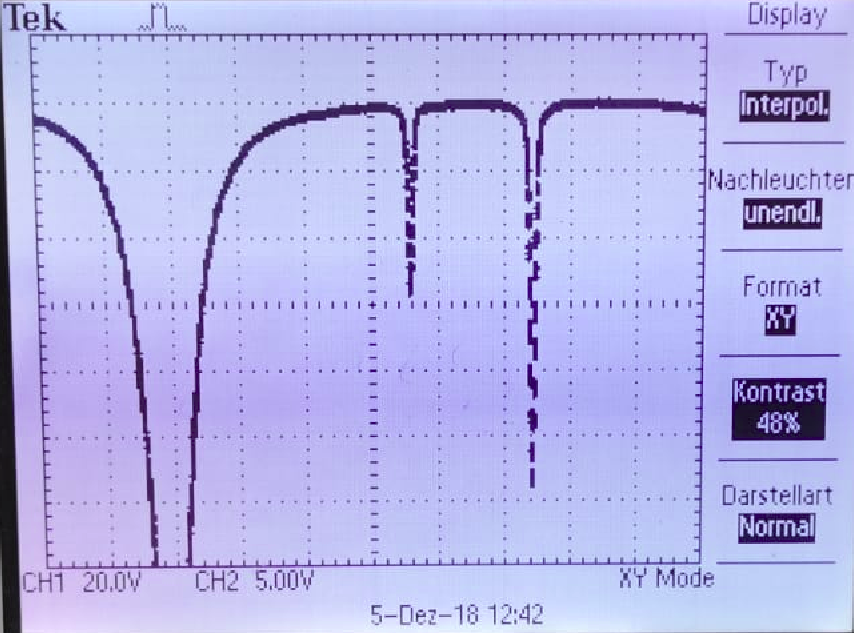
\includegraphics[scale=0.3]{Foto.png}
  \caption{Signalbild mit Resonanzstellen.}
  \label{abb:2}
\end{figure}

Aus dem Amplitudenverhältnis der beiden Resonanzstellen lässt sich auf das
Isotopenverhältnis schließen:
\begin{align*}
  A_1 &= 195\text{px} \\
  A_2 &= 387\text{px} \\
\end{align*}
Damit folgt für die prozentualen Verteilungen $p$:
\begin{align*}
  p_{^{87}\text{Rb}} = \SI{33,5}{\percent} \\
  p_{^{85}\text{Rb}} = \SI{66,5}{\percent} \\
\end{align*}

In der Natur liegen die Isotope in dem folgenden Verhältnis vor : \cite{Q2}
\begin{align*}
  p_{^{87}\text{Rb}, theo} = \SI{28}{\percent} \\
  p_{^{85}\text{Rb}, theo} = \SI{72}{\percent} \\
\end{align*}

\subsection{Abschätzung des quadratischen Zeeman-Effekts}
Zur Abschätzung des quadratischen Zeeman-Effekts wird zunächst der lineare Teil
berechnet, um diesen mit dem quadratischen Teil zu vergleichen. Hierbei wird das
maximal gemessene Feld zur Berechnung genommen ( \SI{144,90}{\micro\tesla} und
\SI{217,27}{\tesla} für die jeweiligen Resonanzstellen). Mit $M_F=3$ für
$^{85}\text{Rb}$ und $M_F=2$ für $^{87}\text{Rb}$ und den
Hyperfeinstrukturaufspaltungen \cite{Q1} lässt sich mittels Gleichung \eqref{eq_qZeeman}
die linearen und quadratischen Teile berechnen:
\begin{align*}
  E_{1, linear} &= \SI{4,21(4)e-9}{\eV} \\
  E_{2, linear} &= \SI{4,186(35)e-9}{\eV} \\
  E_{1, quadratisch} &= \SI{-1,88(4)e-12}{\eV} \\
  E_{2, quadratisch} &= \SI{-6,98(12)e-12}{\eV} \\
\end{align*}

\section{Diskussion}
Das horizontale Erdmagnetfeld hat ist in etwa \SI{20}{\micro\meter} groß \cite{Q3}.

Der Theoriewert liegt im Fehlerintevall unserer Messwerte
(\SI{10(10)}{\micro\tesla} und \SI{9(12)}{\micro\tesla}), jedoch ist der Fehler
bei der Messung sehr groß.

Der Vergleich der Theoriewerte und der Messwerte des Kernspins zeigen nur sehr
geringe Abweichungen von maximal \SI{0,4}{\percent} und die Theoriewerte liegen
in den Fehlerintervallen der Messwerte (siehe Tabelle \ref{tab:diskussion}).
Daraus zeigt sich, dass dies ein sehr genaues Verfahren zu Messung der
Landéschen Faktoren und des Kernspins ist.

\begin{table}
  \centering
  \caption{Vergleich: Theoriewerte und Messwerte des Kernspins}
  \label{tab:diskussion}
  \begin{tabular}{c| c c c}
    \toprule
    Isotop & Theoriewert & Messwert & Abweichung/\si{\percent}\\
    \midrule
    $^{87}\text{Rb}$ & 1,5 &  \num{1,494(21)} & 0,4 \\
    $^{85}\text{Rb}$ & 2,5 &  \num{2,508(25)} & 0,32 \\
    \bottomrule
  \end{tabular}
\end{table}

Die Verteilung der Isotope ist nicht identisch mir der Verteilung der Isotopen
in der Natur. Dieser weicht um etwa 5,5 Prozentpunkte ab.

Bei der Abschätzung des quadratischen Zeeman-Effektes ist zu erkennen, dass sich
die Werte des linearen und des quadratischen Terms um 3 Größenordnungen
unterscheiden (siehe Tabelle \ref{tab:diskussion2}).
Somit kann davon ausgegangen werden, dass der quadratische
Zeeman-Effekt in diesem Versuch vernachlässigt werden kann.

\begin{table}
  \centering
  \caption{Berechnungen der Energie des quadratischen Zeeman-Effektes.}
  \label{tab:diskussion2}
  \begin{tabular}{c c c}
    \toprule
    Isotop & E linearer Term / \si{eV} & E quadratischer Term / \si{\eV} \\
    \midrule
    $^{87}\text{Rb}$ & \num{4,21(4)e-9} & \num{-1,88(4)e-12} \\
    $^{85}\text{Rb}$ & \num{4,186(35)e-9} & \num{-6,98(12)e-12} \\
    \bottomrule
  \end{tabular}
\end{table}

\printbibliography
